\documentclass[10pt]{beamer}
%\documentclass[10pt, handout]{beamer}

% general
\usepackage{hyperref}
\hypersetup{colorlinks=true, citecolor=blue, linkcolor=blue, urlcolor=blue} % you can change colors here
\usepackage{natbib}

% tables and figures
\usepackage{booktabs}
\usepackage{float}

\usepackage{graphicx}
\usepackage[skip=10pt]{caption}
\usepackage{lscape}

\setbeamertemplate{caption}[numbered]

\title{Title of your presentation}
\author{Your name \\ Affiliation}
\date{August, 2018}



\begin{document}

\maketitle


\section{Examples}
  \frame{\tableofcontents  \frametitle{Roadmap}}


\subsection{- Itemization}

\begin{frame}
  \frametitle{Itemization}

Change the font size:
\begin{itemize}
	\item {\footnotesize footnotesize}
	\item {\small small}
	\item {\large large}
	\item {\Large Large}
	\item {\LARGE LARGE}
	\item {\huge huge}
	\item {\Huge Huge}
\end{itemize}

\end{frame}

\subsection{- Math}

\begin{frame}
  \frametitle{Math}

Write a math expression like this $y = f(x)$, or:
\begin{equation}
	y = \alpha + \beta x + \epsilon. \label{eq:reg} 
\end{equation}

\end{frame}


\subsection{- Tables}

\begin{frame}
  \frametitle{Tables}

\begin{table}[H] 
	\caption{Summary statistics}
	\begin{center}
	\scalebox{0.9}[0.9]{
		\begin{tabular}{llllll}
\toprule
{} &      mean &       std &      min &   max & count \\
\midrule
uid           &   1281.48 &   736.896 &        1 &  2538 &  3392 \\
ELECYEAR      &   2011.56 &   1.98969 &     2009 &  2014 &  3392 \\
PREFEC        &   20.8821 &   12.2485 &        1 &    47 &  3392 \\
DISTRICT      &   5.77712 &   5.13715 &        1 &    25 &  3392 \\
PRBLOCK       &   58.8544 &   5.09346 &       51 &    66 &  2906 \\
INCUMB        &   1.79658 &  0.938328 &        1 &     3 &  3392 \\
TERM          &   1.45136 &   2.39026 &        0 &    16 &  3392 \\
SEX           &   1.15271 &  0.359763 &        1 &     2 &  3392 \\
AGE           &   50.5746 &   11.2587 &       25 &    94 &  3390 \\
RESULT        &    2.0339 &    1.2166 &        1 &     4 &  3392 \\
\bottomrule
\end{tabular}

	}
	\end{center}
\end{table}
{\footnotesize {\it Notes}: Brabrabra.}

\end{frame}


\subsection{- Figures}

\begin{frame}
  \frametitle{Figures}

\begin{figure}[H]
	\begin{center}
	\caption{Political candidates' opinion about fiscal policy, by sex} 
	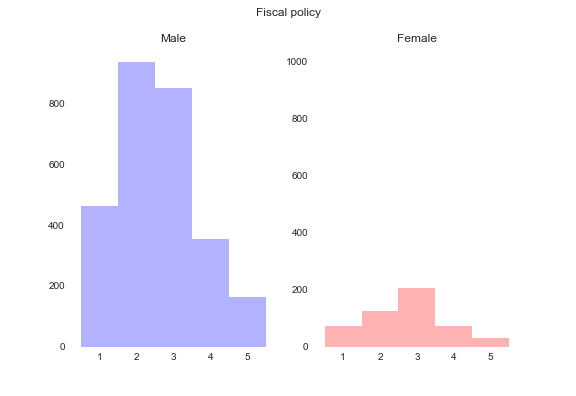
\includegraphics[width=0.8\textwidth]{yn_fiscalpol_bysex_py.png} \label{fig:hist2} 
	\end{center}
	\vspace{-5mm}
\end{figure}
{\footnotesize {\it Notes}: Brabrabra.}

\end{frame}


\end{document}